\section{Estimation and Simulation procedureS} \label{sec:estimation-evaluation-simulation}


This section presents computational aspects of the estimation of our proposed model, such as the mathematical programming formulation that accounts for the two regularization terms introduced in previous sections. We also present the algorithm to perform a Monte Carlo simulation with the estimated model and an out-of-sample procedure to determine the best regularization parameters. The methodology is implemented in R \cite{rlanguage2008} and Julia \cite{bezanson2012julia} languages, using  packages JuMP \cite{DunningHuchetteLubin2017}, Gurobi, RCall and Dierckx. 


\subsection{Estimation of the QRAL model} \label{sec:qral-estimation}

We assume that all covariates are normalized. If they are not in the same scale, the shrinkage feature of the LASSO will fail, as different variables may have different weights according to their relative size. Thus, let $\tilde x_{t,p}$ be an input observation at time $t$ of covariate variable $p$.
The normalization process is a linear transformation to each covariate $p$, such that all have a mean of $0$ and a variance of $1$. 
We apply the transformation ${x}_{t,p} = (\tilde x_{t,p} - \bar{x}_{p}) / \hat\sigma_{\tilde x_{p}}$, where $\bar{x}_{p}$ and $\hat{\sigma}_{\tilde x_{p}}$ are the covariate $p$'s unconditional mean and standard deviation, respectively. The response variable $Y$ does not need to be transformed.

The QRAL model, as described in problem (\ref{eq:adaLASSO_model_mat1})-(\ref{eq:adaLASSO_model_mat2}), can be implemented as a linear programming problem as shown below:
\begin{IEEEeqnarray}{lr}
	\underset{\beta_{0},\beta,\varepsilon_{t j}^{+},\varepsilon_{t j}^{-}}{\text{min}} \sum_{j \in J} \sum_{t \in T}(\alpha_j\varepsilon_{t j}^{+}+(1-\alpha_j)\varepsilon_{t j}^{-}) \span \nonumber  \\
	\span + \lambda \sum_{p \in P} \sum_{j \in J} w_{pj} (\xi^+_{pj} + \xi^-_{pj}) \nonumber \\ 
	\span + \gamma \sum_{p \in P} \sum_{j \in J'} (D2_{pj}^+ + D2_{pj}^-),  \label{eq:adaLASSO-1} \\
	\mbox{subject to:} \nonumber & \\
	\varepsilon_{t j}^{+}-\varepsilon_{t j}^{-}=y_{t}-\beta_{0 j}-\beta_{j}^T x_{t},& \forall t \in T ,\forall j \in J,\\
	\xi_{pj}^+ - \xi_{pj}^- = \beta_{pj},&\forall p \in P, \forall j \in J\\ 
	D2_{pj}^+ - D2_{pj}^- = \frac{\left(\frac{\beta_{p,j+1}-\beta_{pj}}{\alpha_{j+1}-\alpha_{j}}\right)-\left(\frac{\beta_{p,j}-\beta_{p,j-1}}{\alpha_{j}-\alpha_{j-1}}\right)}{\alpha_{j+1}-\alpha_{j-1}}, \span   \nonumber \\
	\span \forall p\in P, \forall j \in J',  \\
	\beta_{0j} + \beta_{j}^T x_{t} \leq \beta_{0,j+1} + \beta_{j+1}^T x_{t},&\forall t \in T, \forall j \in J_{(-1)}, \label{eq:qral-crossing} \\
	\varepsilon_{t j}^{+},\varepsilon_{t j}^{-}\geq0,&\forall t \in T, \forall j \in J,\\
	\xi_{pj}^+, \xi_{pj}^- \geq 0, & \forall p\in P, \forall j \in J, \\
	D2_{pj}^+, D2_{pj}^- \geq 0, & \forall p\in P, \forall j \in J'. \label{eq:adaLASSO-ult} 
\end{IEEEeqnarray}

Variables $\varepsilon^+_t$ and $\varepsilon^-_t$ represent the quantities $|y-q(\cdot)|^+$ and $|y-q(\cdot)|^-$, respectively. The first line on the objective function in (\ref{eq:adaLASSO-1}) represents the sum of the function $\rho$ over all $j$, i.e., $ \rho_{\alpha_j}(y-q(\cdot)) = \alpha_j \varepsilon^+_{tj} + (1-\alpha_j) \varepsilon^-_{tj}$. The second derivative term $D^2_{\alpha_j}\beta_{pj}$ is implemented on the optimization problem by adding a penalty on the objective function to penalize its absolute value, modeled as the sum of auxiliary variables $D2_{pj}^+ + D2_{pj}^-$. The tuning parameter $\gamma$ controls how rough the sequence $\{\beta_{pj}\}_{j \in J}$ can be, for a given $p$.


% \subsection{Time-series Cross Validation} \label{sec:cv}

% Estimating the QRAL involves parameters $\lambda$ and $\gamma$, which should be known \textit{a priori}. In statistics and machine learning, a popular technique is using cross-validation (CV) to select the best value of parameters from the range of possibilities. How to select their values among this range is a crucial point in our methodology, as the estimated coefficients vary considerably with respect to parameter choice.

% Out of the different possible implementations of CV, we use the $\mathcal{K}$-fold CV. It consists in first partitioning the dataset in $\mathcal{K}$ equally sized sets, which are the $\mathcal{K}$ folds. For each fold $k \in \{1,\dots,\mathcal{K}\}$, the remaining $\mathcal{K}-1$ folds are used to estimate the model using parameter $\theta$ (for the QRAL model, $\theta = [\gamma \quad \lambda]^T$) and predicting the values in fold $k$. The error function $MAPE_\theta$ measures the result of this prediction.
% So, the CV error is given by the sum of all folds, for a given model which uses the vector of parameter $\theta$ is given by
% \[
%  CV(\theta) = \sum_{k \in \mathcal{K}} \sum_{j \in J} MAPE_\theta.\label{eq:cv-error}
% \]
% The optimum parameter $\theta^*_{CV}$, according to this methodology, is the value of $\theta$ which minimizes the CV error
% \begin{equation}
% \theta_{CV}^* = \argmin_\theta CV(\theta) .\label{eq:cv-equation}
% \end{equation}

% The usage of CV is not straightforward when data is dependent, which is the case of time series. As it is time dependent, one can be interested in using either all observations or to take the dependence away to not interfere on the estimation. The works
% \cite{bergmeir_note_2017} and \cite{bergmeir_use_2012} deals specifically with the usage of CV in a time series context. They provide tests with both $\mathcal{K}$-fold CV and $\mathcal{K}$-fold with non-dependent data. Both schemes are shown of Figure \ref{fig:cross-validation-scheme}.
% \begin{figure}
% 	\centering
% 	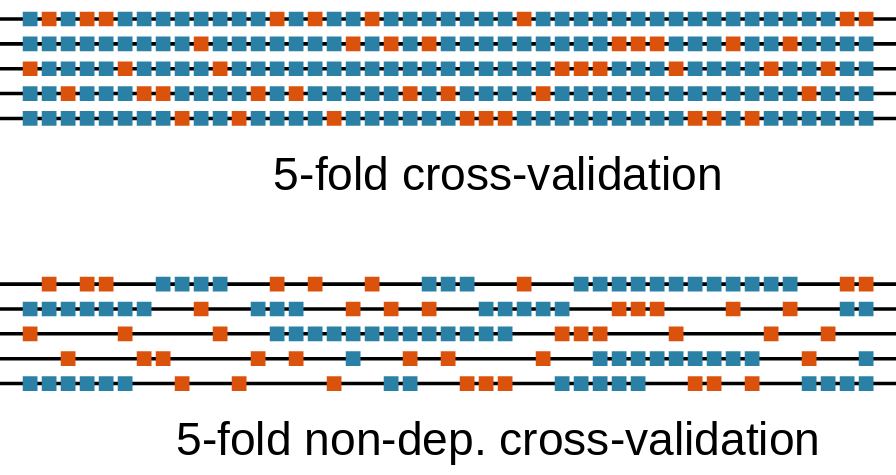
\includegraphics[width=0.7\linewidth]{Images/Cross-validation-scheme}
% 	\caption{$\mathcal{K}$-fold CV and $\mathcal{K}$-fold with non-dependent data. Observations in blue are used to estimation and in orange for evaluation. Note that non-dependent data does not use all dataset in each fold. Image from \cite{bergmeir_note_2017}.}
% 	\label{fig:cross-validation-scheme}
% \end{figure}
% In both settings, the training data is randomly split into a collection of sets $S_k$, forming a $\mathcal{K}$ size partition. Each of these $S_k$ is used as test set, while the rest is used to estimate coefficients which will be used to predict values of $S_k$. 
% As there are $\mathcal{K}$ folds, this procedure is done $\mathcal{K}$ times. 
% So, for a given vector of tuning parameter $\theta$, the CV score is given by the sum of the error function for each fold. 
% As the CV score is nonconvex, the optimization in (\ref{eq:cv-equation}) is done by iterating over a sequence of values in a thin grid and choosing the smallest one.




% Even though CV is very popular and produce great results, selecting model with Information Criteria involves less computational time. For the case where the selected model is very similar, it might be the case that the estimation methodology may change a little bit. It is definitely a topic that worths researching.


% \todoi{Ver se novas figuras (R/grafico-cv.r) e ver se incluir outras formas de CV} % escolhemos trabalhar apenas com este tipo de CV





\subsection{Monte Carlo scenario generation} \label{sec:scenario-generation}

%Let $|T|$ be the total length of $\{y_t\}$ and $S$ the number of scenarios of size $K$ we produce. 
%The variables chosen to compose $x_t$ can be either exogenous variables, autoregressive components of $y_t$ or both. We use a nonparametric approach which to estimate, at every $t$, the $k$-step ahead conditional density of $y_t$.
We use a Monte Carlo (MC) approach to produce $S$ different future scenarios $\{ \hat{y}_{\tau,s} \}_{\tau=|T|+1}^{|T|+K}$ of length $K$. It consists of first estimating the model for a given time $\tau$ and scenario $s$. Then, for each of these we take the input vector $x_{\tau,s}$ and calculate the discrete quantile function $\tilde{Q}_{y_{\tau}|X}$, which is an intermediate step to estimate the continuous quantile function $\hat{Q}_{y_{\tau}|X}$. 
This same MC procedure is employed to produce scenario simulations for a variety of QR-based models, including the QRAL. This procedure is detailed in Algorithm \ref{alg:mc-procedure}.

\begin{algorithm}
% \noindent\rule{\columnwidth}{1pt}

\caption{MC procedure for simulating $S$ scenarios $K$ steps ahead}
\label{alg:mc-procedure}
% \noindent\rule{\columnwidth}{1pt}

\begin{enumerate}
	
	\item Estimate a QR model (for the QRAL solve the optimization problem defined in equation (\ref{eq:adaLASSO-1})-(\ref{eq:adaLASSO-ult})). 
	A set of coefficients $\{ \hat\beta_{0j} \}_{j \in J}$ and $\{ \hat\beta_{j} \}_{j \in J}$ is the output from this optimization, using time series $y_t$ and $x_{pt}$ from the period $t = 1, \dots, |T|$. 

	\item Initialize time index $\tau = |T| + 1$.
	
	\item For each scenario $s \in S$, do:
		\begin{enumerate}

		\item Let $x_{\tau,s} = [y_{\tau-1,s}, \dots, y_{\tau-24,s}]$ be the vector of explanatory variables used as the input to predict the conditional distribution function in time $\tau$ and scenario $s$.

		\item Let $\tilde{Q}_{y_{\tau}|X}:A \times \mathbb{R}^d \rightarrow \mathbb{R}$ be the discrete quantile function. Its values are mapped according to the estimated quantile $\tilde Q_{y_{\tau}|X}(\alpha_j, x_{\tau,s}) \leftarrow \hat\beta_{0j} + \hat\beta_j^T x_{\tau,s}$, for all $j \in J$.
		
		\item To define the continuous function $\hat{Q}_{y_{\tau}|X}:[0,1] \times \mathbb{R}^d \rightarrow \mathbb{R}$ from $\tilde Q_{y_{\tau}|X}$, use a linear interpolation to connect the points. As $0 < \alpha_1 < \cdots < \alpha_{|J|} < 1$, there are no quantile estimates for the intervals $[0,\alpha_1]$ and $[\alpha_{|J|},1]$. These gaps are filled by linearly extending the line that connects $\alpha_1$ to $\alpha_2$ on the left hand side and extending the line that connects $\alpha_{|J|-1}$ to $\alpha_{|J|}$ on the right hand side until the support $[0,1]$ is fully mapped.  

		% \item In any given period $\tau$, for every $\alpha \in A$, we estimate $q_{\alpha_{j}}$, for every $j \in J$.
		% Note that $x_{\tau}$ is supposed to be known at time $\tau$\footnote{In the presence of exogenous variables that are unknown, it is advisable to incorporate its uncertainty by considering different scenarios. In each scenario, though, $x_{\tau}$ must be considered fully known.}.
		
		% \item Let $\hat{Q}_{y_{\tau,s}|X}(\alpha,x_\tau)$ be the estimated quantile function of ${y}_{\tau,s}$. 
		% At first, we define a discrete quantile function $\tilde{Q}_{y_{\tau,s}}$. By mapping every $\alpha \in A$ with its estimated quantile $\hat{q}_{\alpha_j}(x_t)$, we define function $\tilde{Q}_{y_{\tau,s}}$. In order to produce a continuous function from a set of ordered points, we use linear interpolation and we arrive on the Quantile function $\hat{Q}_{y_{\tau}}$.
		
		%This process is described in more details on section \ref{sec:estimating-distribution}. 
		\item Let $U$ be a random variable with a uniform distribution over the interval $[0,1]$. As $Q_{y_\tau}(U)$ has the same distribution as $y_\tau$, by taking
		$$y_{\tau,s} \leftarrow \hat Q_{y_\tau | X}(u), \quad u \sim U[0,1],$$
		we simulate scenarios next values.



		 \end{enumerate}
	% let $x_{\tau,s} = [y_{\tau-1,s}, \dots, y_{\tau-12,s}]$ be the vector of explanatory variables, used as input to predict the conditional distribution function in time $\tau$ and scenario $s$.
	
	
	\item Let $\tau = \tau + 1$. If $\tau > K$, then stop. Else, go back to step 3) . 


\end{enumerate}

% \noindent\rule{\columnwidth}{1pt}
\end{algorithm}


\subsection{Estimating the regularization parameters} \label{sec:SIC}

% Most statistical models are designed to provide a good fit on point forecasts. In this work, however, the objective is to produce a predictive CDF. To evaluate the statistical quality of a given pair of regularization parameters ($\lambda$ and $\gamma$), the estimated CDF is compared with the actual observed data one-step ahead within a rolling horizon out-of-sample test. To do that, the difference between the quantile probability forecast $\alpha_j$ and its actual frequency of occurrence $f_j$ is computed for an out-of-sample set of data. While $\alpha_j$ is given by the model specification, $f_j$ is computed based on the number of observations belonging to the quantile interval $(q_{\alpha_{j-1}}(x_t), q_{\alpha_{j}}(x_t)]$ along the experiment.


% The mean absolute error (MAE) of the conditional quantiles forecast and observed ones for a given out-of-sample horizon $H$ is defined by
% \begin{equation}
% MAE_{\theta}= \frac{1}{|J|} \sum_{j \in J} \left| \alpha_j -  f_j  \right|.
% \label{eq:MAE}
% \end{equation}



Most statistical models are designed to provide a good fit on point forecasts. In this work, however, the objective is to produce a predictive CDF. To evaluate the statistical quality of a given pair of regularization parameters ($\lambda$ and $\gamma$), the estimated CDF is compared with the actual observed data one-step ahead within a rolling horizon out-of-sample test. To do that, the difference between the quantile probability forecast $\alpha_j$ and its actual cumulative frequency of occurrence $F_j$ is computed for an out-of-sample set of data. While $\alpha_j$ is given by the model specification (or, in case of assessing the performance $K$ steps ahead, by simulation using Algorithm \ref{alg:mc-procedure}), $F_j$ is computed based on the number of observations belonging to the quantile interval $(q_{\alpha_{j-1}}(x_t), \infty)$ along the experiment.


The mean absolute error (MAE) of the conditional quantiles forecast and observed ones for a given out-of-sample horizon $H$ is defined by
\begin{equation}
MAE_{\theta}= \frac{1}{|J|} \frac{1}{|H|}  \sum_{j \in J} \sum_{t \in H} \left| \alpha_j -  F_{tj}  \right|,
\label{eq:MAE}
\end{equation}
where $F_{tj}$ is the cumulative frequency at time $t$.

%where $q_t^{\alpha_{j}}$ is the unconditional $\alpha_j$-quantile  and $\hat q_t^{\alpha_j}$ is the predicted $\alpha_j$-quantile. We obtain $q_t^{\alpha_j}$ by taking the $\alpha_j$-quantile of the historic values of a given month. The predicted $\hat q_t^{\alpha_j}$ is obtained by taking the $\alpha_j$-quantile. 
The MAE function emphasizes the estimated CDF accuracy across the quantiles for data not seen before. Depending on the application, it might be interesting to put different weights on different quantiles. In this work, however, we will treat every quantile as equal concerning the error measure.



Another relevant metric, largely used in time-series analysis as the state-of-the art model selection tool, is the Information Criteria (IC). It is also employed in other multiple quantile model studies \cite{zou_regularized_2008, jiang_interquantile_2014} to tune parameters. An IC summarizes two desirable characteristics in model selection: in-sample goodness of fit and penalization of complexity (or lack of parsimonity) as given by the model size. Hence, in order for a covariate to be included in the model, it must supply a sufficient goodness of fit. The expression for SIC appropriate for quantile autoregression is presented below:

 \begin{equation} 
\small
SIC_\theta = \sum_{j \in J} \left( \log \left(\sum_{t \in T}\rho_{\alpha_j}(y_t - \beta_{0j}^\theta - \beta_j^{T\theta} x_t) \right) +  \frac{\log(|T|)|\epsilon_\theta|}{2|T|}  \right),\label{eq:SIC}
\end{equation}
where $\theta = [\gamma \quad \lambda]^T$ and $\epsilon_\theta$ is the elbow set, defined as $\epsilon_\theta = \{(t,j): y_t - q_{\alpha_j}(x_t) = 0 \}$. The authors in \cite{li_l1-norm_2008} show that the quantity $|\epsilon_\theta|$ is the effective degrees of freedom in the quantile regression.







